\documentclass[aspectratio=169,10pt]{beamer}
\usetheme{Madrid}
\usecolortheme{default}
\usepackage{fontspec}
\setmainfont{Times New Roman}
\setsansfont{Arial}
\usepackage{booktabs}
\usepackage{graphicx}
\usepackage{array}
\usepackage{tabularx}
\usepackage{tikz}
\graphicspath{{../../outputs/figures/}{../figures/}}
\setbeamertemplate{navigation symbols}{}
\setbeamertemplate{caption}[numbered]
\setbeamertemplate{itemize items}[circle]
\definecolor{FreshGreen}{RGB}{31,121,74}
\definecolor{FreshDark}{RGB}{22,78,99}
\setbeamercolor{structure}{fg=FreshGreen}
\setbeamercolor{frametitle}{fg=white,bg=FreshGreen}
\setbeamercolor{title}{fg=white,bg=FreshGreen}
\setbeamercolor{block title}{fg=white,bg=FreshDark}
\setbeamercolor{block body}{bg=gray!6}

\title[FreshRetailNet-50K]{Dự báo chuỗi thời gian bán lẻ có xét đến tình trạng hết hàng}
\subtitle{Two-stage latent demand recovery + daily demand forecasting trên FreshRetailNet-50K}
\author{Nhóm 3}
\date{}

\begin{document}

\begin{frame}
    \titlepage
\end{frame}

\begin{frame}{Mục lục trình bày}
    \begin{columns}[T]
        \begin{column}{0.48\linewidth}
            \begin{enumerate}
                \item Introduction
                \item Dataset \& EDA
                \item Methodology
                \item Forecasting Results
            \end{enumerate}
        \end{column}
        \begin{column}{0.48\linewidth}
            \begin{enumerate}
                \setcounter{enumi}{4}
                \item Model Evaluation
                \item Business Insights
                \item Conclusion
                \item Future Work
            \end{enumerate}
        \end{column}
    \end{columns}
    \vspace{0.25cm}
    \begin{block}{Thông điệp chính}
    Với dữ liệu bán lẻ có stockout, forecast trực tiếp observed sales dễ học sai nhu cầu. Đồ án xử lý bằng pipeline two-stage: recover latent demand theo giờ, rồi forecast daily next-7-day demand.
    \end{block}
\end{frame}

\section{Introduction}
\begin{frame}{1. Introduction: bài toán không chỉ là forecast sales}
    \begin{block}{Vấn đề cốt lõi}
    Observed sales có thể bị \textbf{censor} bởi stockout: bán thấp không chắc là nhu cầu thấp, mà có thể là cửa hàng không còn hàng để bán.
    \end{block}
    \begin{columns}[T]
        \begin{column}{0.49\linewidth}
            \textbf{Nếu forecast trực tiếp observed sales}
            \begin{itemize}
                \item Model học cả nhu cầu thật lẫn giới hạn tồn kho.
                \item Dễ under-forecast ở nhóm hay hết hàng.
                \item Vòng lặp xấu: dự báo thấp $\rightarrow$ nhập ít $\rightarrow$ tiếp tục stockout.
            \end{itemize}
        \end{column}
        \begin{column}{0.49\linewidth}
            \textbf{Hướng của đồ án}
            \begin{itemize}
                \item Recover latent demand ở các giờ stockout.
                \item Aggregate hourly recovered demand lên daily.
                \item Forecast tổng demand 7 ngày tiếp theo.
            \end{itemize}
        \end{column}
    \end{columns}
\end{frame}

\begin{frame}{Câu hỏi nghiên cứu và contribution}
    \begin{enumerate}
        \item Có thể recover demand bị che trong stockout mà không leakage thời gian không?
        \item Imputation có làm tổng demand tăng quá mức không?
        \item Forecast trên recovered demand có tốt hơn forecast trên observed sales không?
        \item Các kết quả này chuyển thành insight vận hành như thế nào?
    \end{enumerate}
    \vspace{0.2cm}
    \begin{columns}[T]
        \begin{column}{0.49\linewidth}
            \textbf{Đóng góp kỹ thuật}
            \begin{itemize}
                \item Expanding-window recovery.
                \item Calibration + cap q90.
                \item Pseudo-stockout validation.
                \item Hybrid seasonal-ML.
            \end{itemize}
        \end{column}
        \begin{column}{0.49\linewidth}
            \textbf{Đóng góp business}
            \begin{itemize}
                \item Ước lượng lost sales.
                \item Giữ weekly seasonality làm baseline vận hành.
                \item Đề xuất workflow replenishment có uncertainty.
            \end{itemize}
        \end{column}
    \end{columns}
\end{frame}

\section{Dataset \& EDA}
\begin{frame}{2. Dataset: FreshRetailNet-50K sample}
    \begin{columns}[T]
        \begin{column}{0.48\linewidth}
            \begin{tabular}{lr}
                \toprule
                Sample fraction & 10.00\% \\
                Hourly rows & 11,640,000 \\
                Series & 5,000 \\
                Stores & 866 \\
                Products & 516 \\
                Stockout row rate & 24.65\% \\
                \bottomrule
            \end{tabular}
            \vspace{0.25cm}
            \begin{itemize}
                \item Daily rows chứa \texttt{hours\_sale} và \texttt{hours\_stock\_status}.
                \item Disaggregate daily $\rightarrow$ hourly để xử lý stockout đúng cấp.
            \end{itemize}
        \end{column}
        \begin{column}{0.50\linewidth}
            \includegraphics[width=\linewidth]{data_preprocessing_pipeline.png}
        \end{column}
    \end{columns}
\end{frame}

\begin{frame}{EDA: stockout là vấn đề trung tâm}
    \begin{columns}[T]
        \begin{column}{0.50\linewidth}
            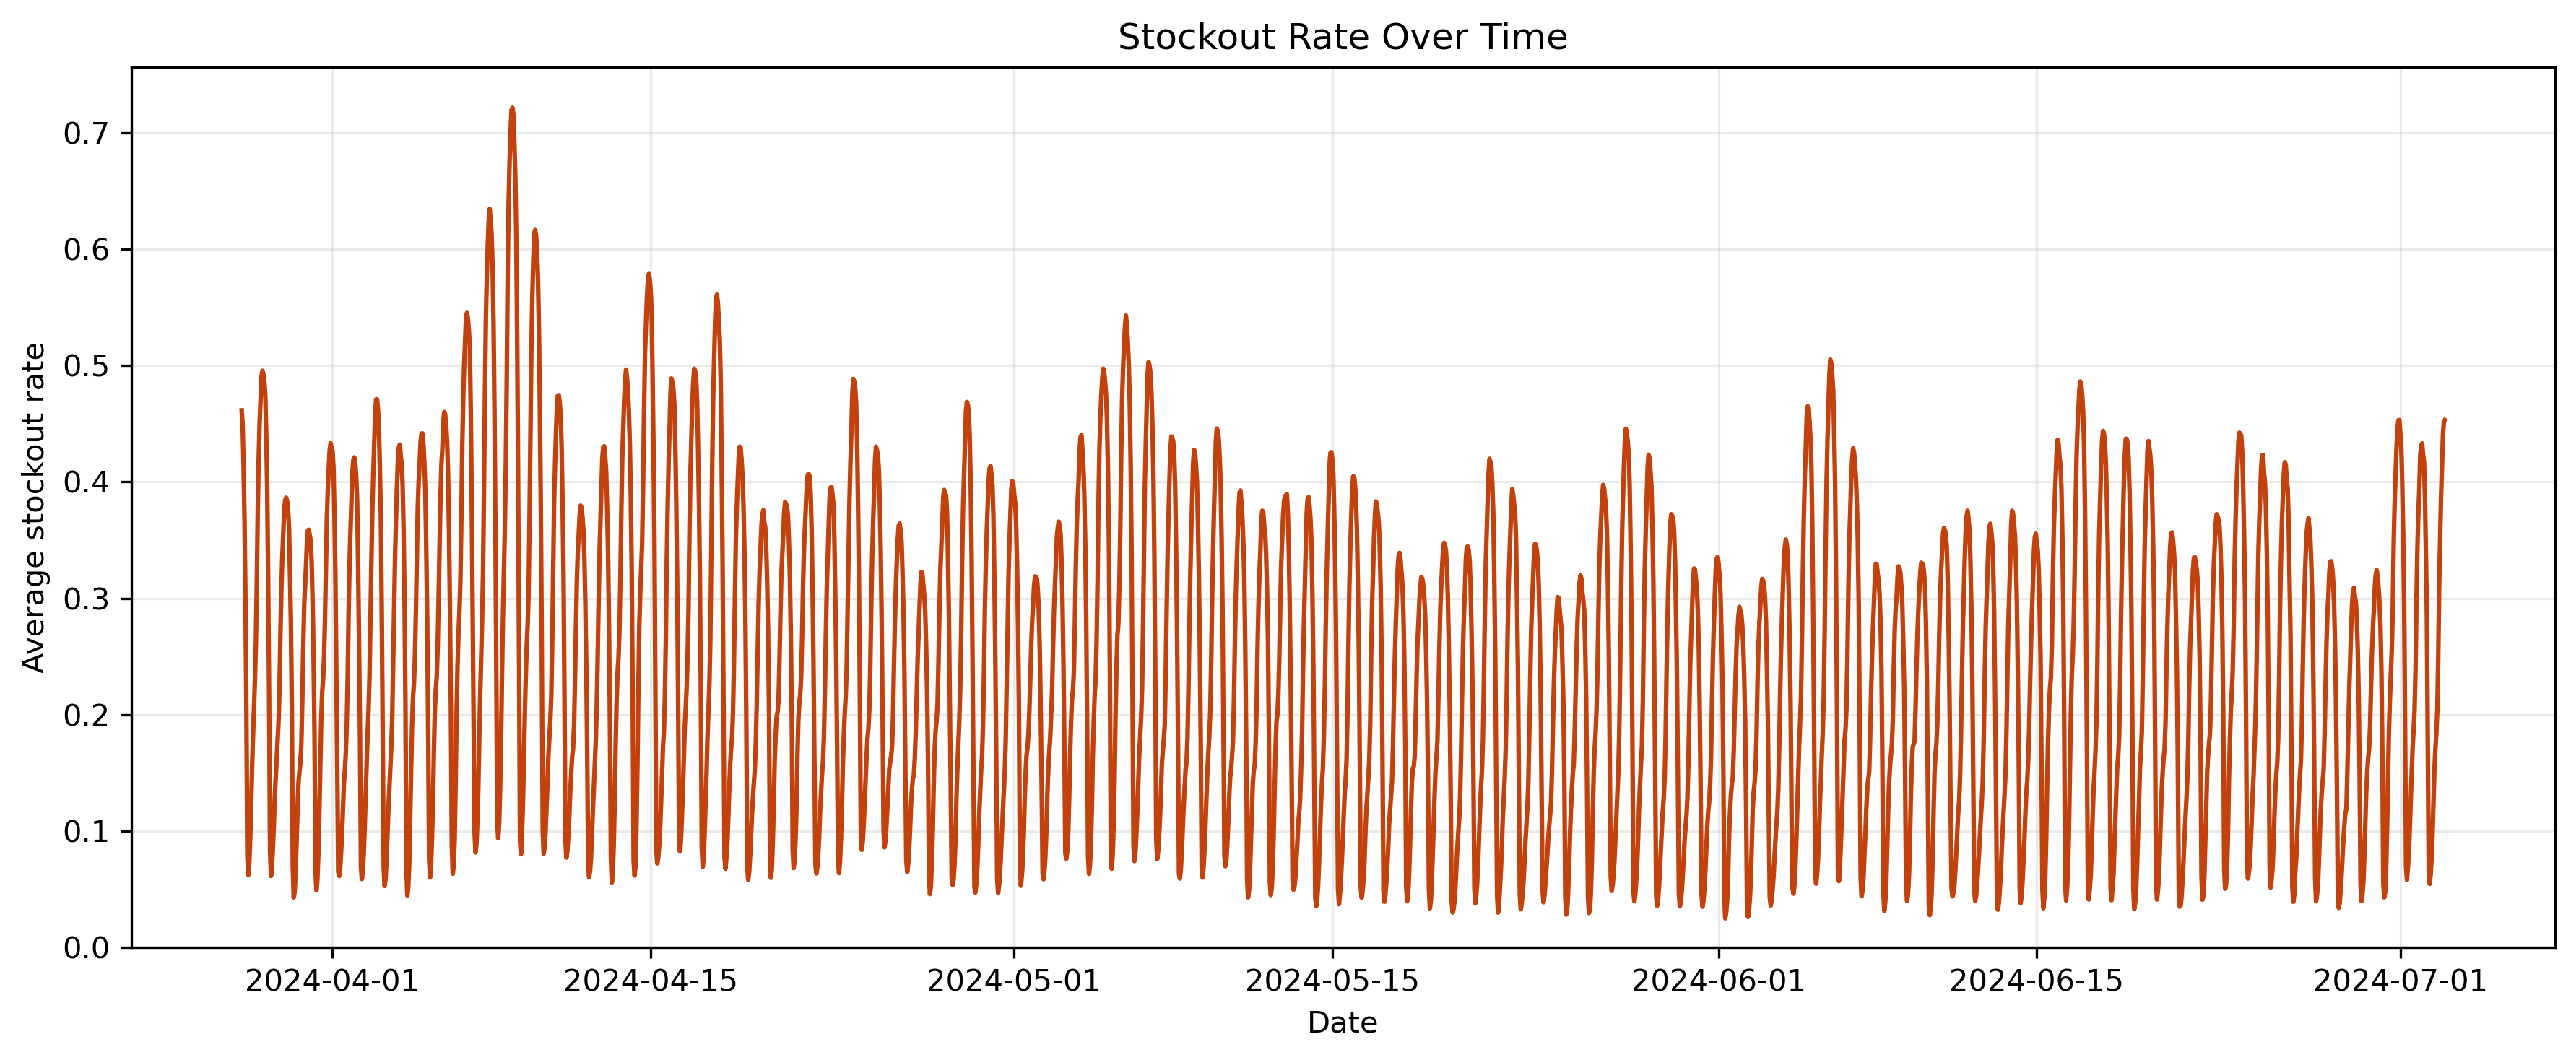
\includegraphics[width=\linewidth]{stockout_rate_over_time.png}
        \end{column}
        \begin{column}{0.47\linewidth}
            \textbf{Hàm ý}
            \begin{itemize}
                \item Stockout rate khoảng 24.65\%.
                \item Đây không phải nhiễu nhỏ để bỏ qua.
                \item Observed sales cần được đọc là dữ liệu có thể bị kiểm duyệt.
            \end{itemize}
            \vspace{0.15cm}
            \begin{block}{Framing}
            Target cuối không phải raw sales, mà là recovered demand proxy có kiểm soát.
            \end{block}
        \end{column}
    \end{columns}
\end{frame}

\begin{frame}{EDA: dữ liệu thưa, lệch và có mùa vụ}
    \begin{columns}[T]
        \begin{column}{0.49\linewidth}
            
\includegraphics[width=\linewidth]{log_sale_amount_distribution.png}
            \begin{itemize}
                \item Nhiều zero, spike và phân phối lệch.
                \item WAPE phù hợp hơn MAPE.
            \end{itemize}
        \end{column}
        \begin{column}{0.49\linewidth}
            
\includegraphics[width=\linewidth]{sales_by_day_of_week.png}
            \begin{itemize}
                \item Weekly seasonality rõ.
                \item Seasonal naive 7-day là benchmark bắt buộc.
            \end{itemize}
        \end{column}
    \end{columns}
\end{frame}

\begin{frame}{ACF/PACF và spectrum dùng để làm gì?}
    \begin{columns}[T]
        \begin{column}{0.50\linewidth}
            
\includegraphics[width=\linewidth]{acf_aggregate_sales.png}
        \end{column}
        \begin{column}{0.47\linewidth}
            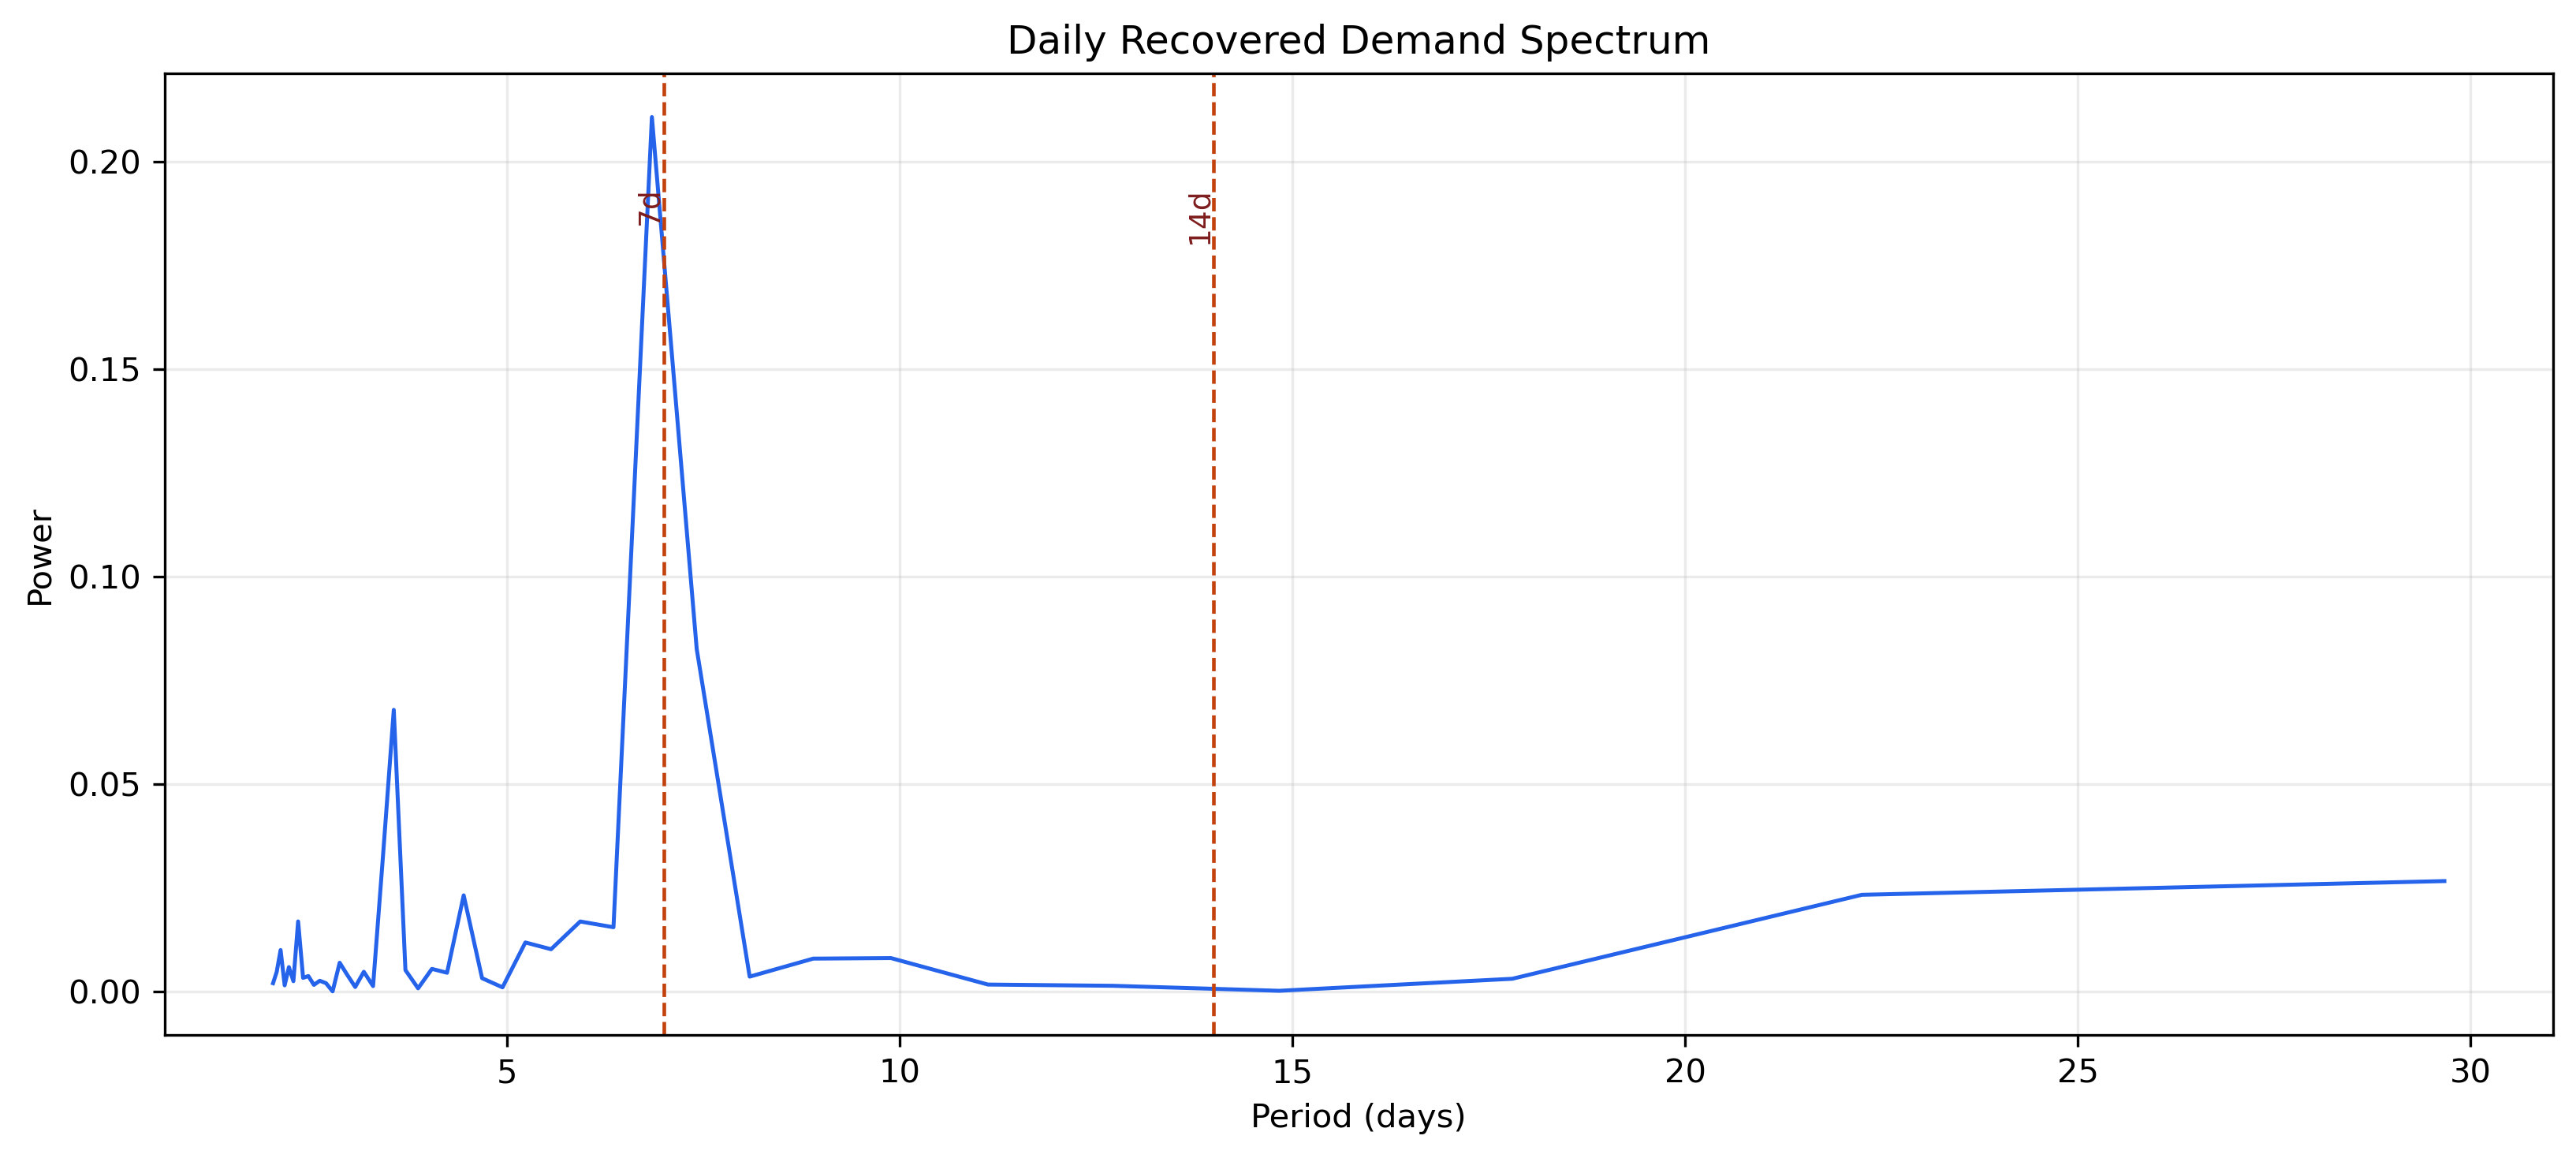
\includegraphics[width=\linewidth]{spectrum_daily_recovered_demand.png}
        \end{column}
    \end{columns}
    \vspace{0.1cm}
    \begin{block}{Cách dùng trong bài}
    Không dùng ACF/PACF để ép chọn ARIMA. Dùng chúng để biện minh lag/rolling/seasonal features và baseline mùa vụ.
    \end{block}
\end{frame}

\begin{frame}{Tại sao không chọn classical time series làm model chính?}
    \begin{columns}[T]
        \begin{column}{0.50\linewidth}
            \textbf{ARIMA/SARIMA từng chuỗi}
            \begin{itemize}
                \item Khó scale cho 5.000 series sample, 50.000 series full.
                \item Không ổn với chuỗi thưa, zero-inflated.
                \item Khó đưa stockout, promotion, weather, category.
            \end{itemize}
        \end{column}
        \begin{column}{0.50\linewidth}
            \textbf{Deep learning}
            \begin{itemize}
                \item Có thể dùng nhưng cần tuning/tài nguyên lớn.
                \item Rủi ro khó bảo vệ nếu validation chưa cực chặt.
                \item Đồ án ưu tiên pipeline rõ, nhẹ, tái lập.
            \end{itemize}
        \end{column}
    \end{columns}
    \vspace{0.2cm}
    \begin{block}{Lựa chọn chính}
    LightGBM global model + seasonal baseline: cân bằng giữa hiệu suất, tốc độ, giải thích và tính tái lập.
    \end{block}
\end{frame}

\section{Methodology}
\begin{frame}{3. Methodology: two-stage framework}
    \centering
    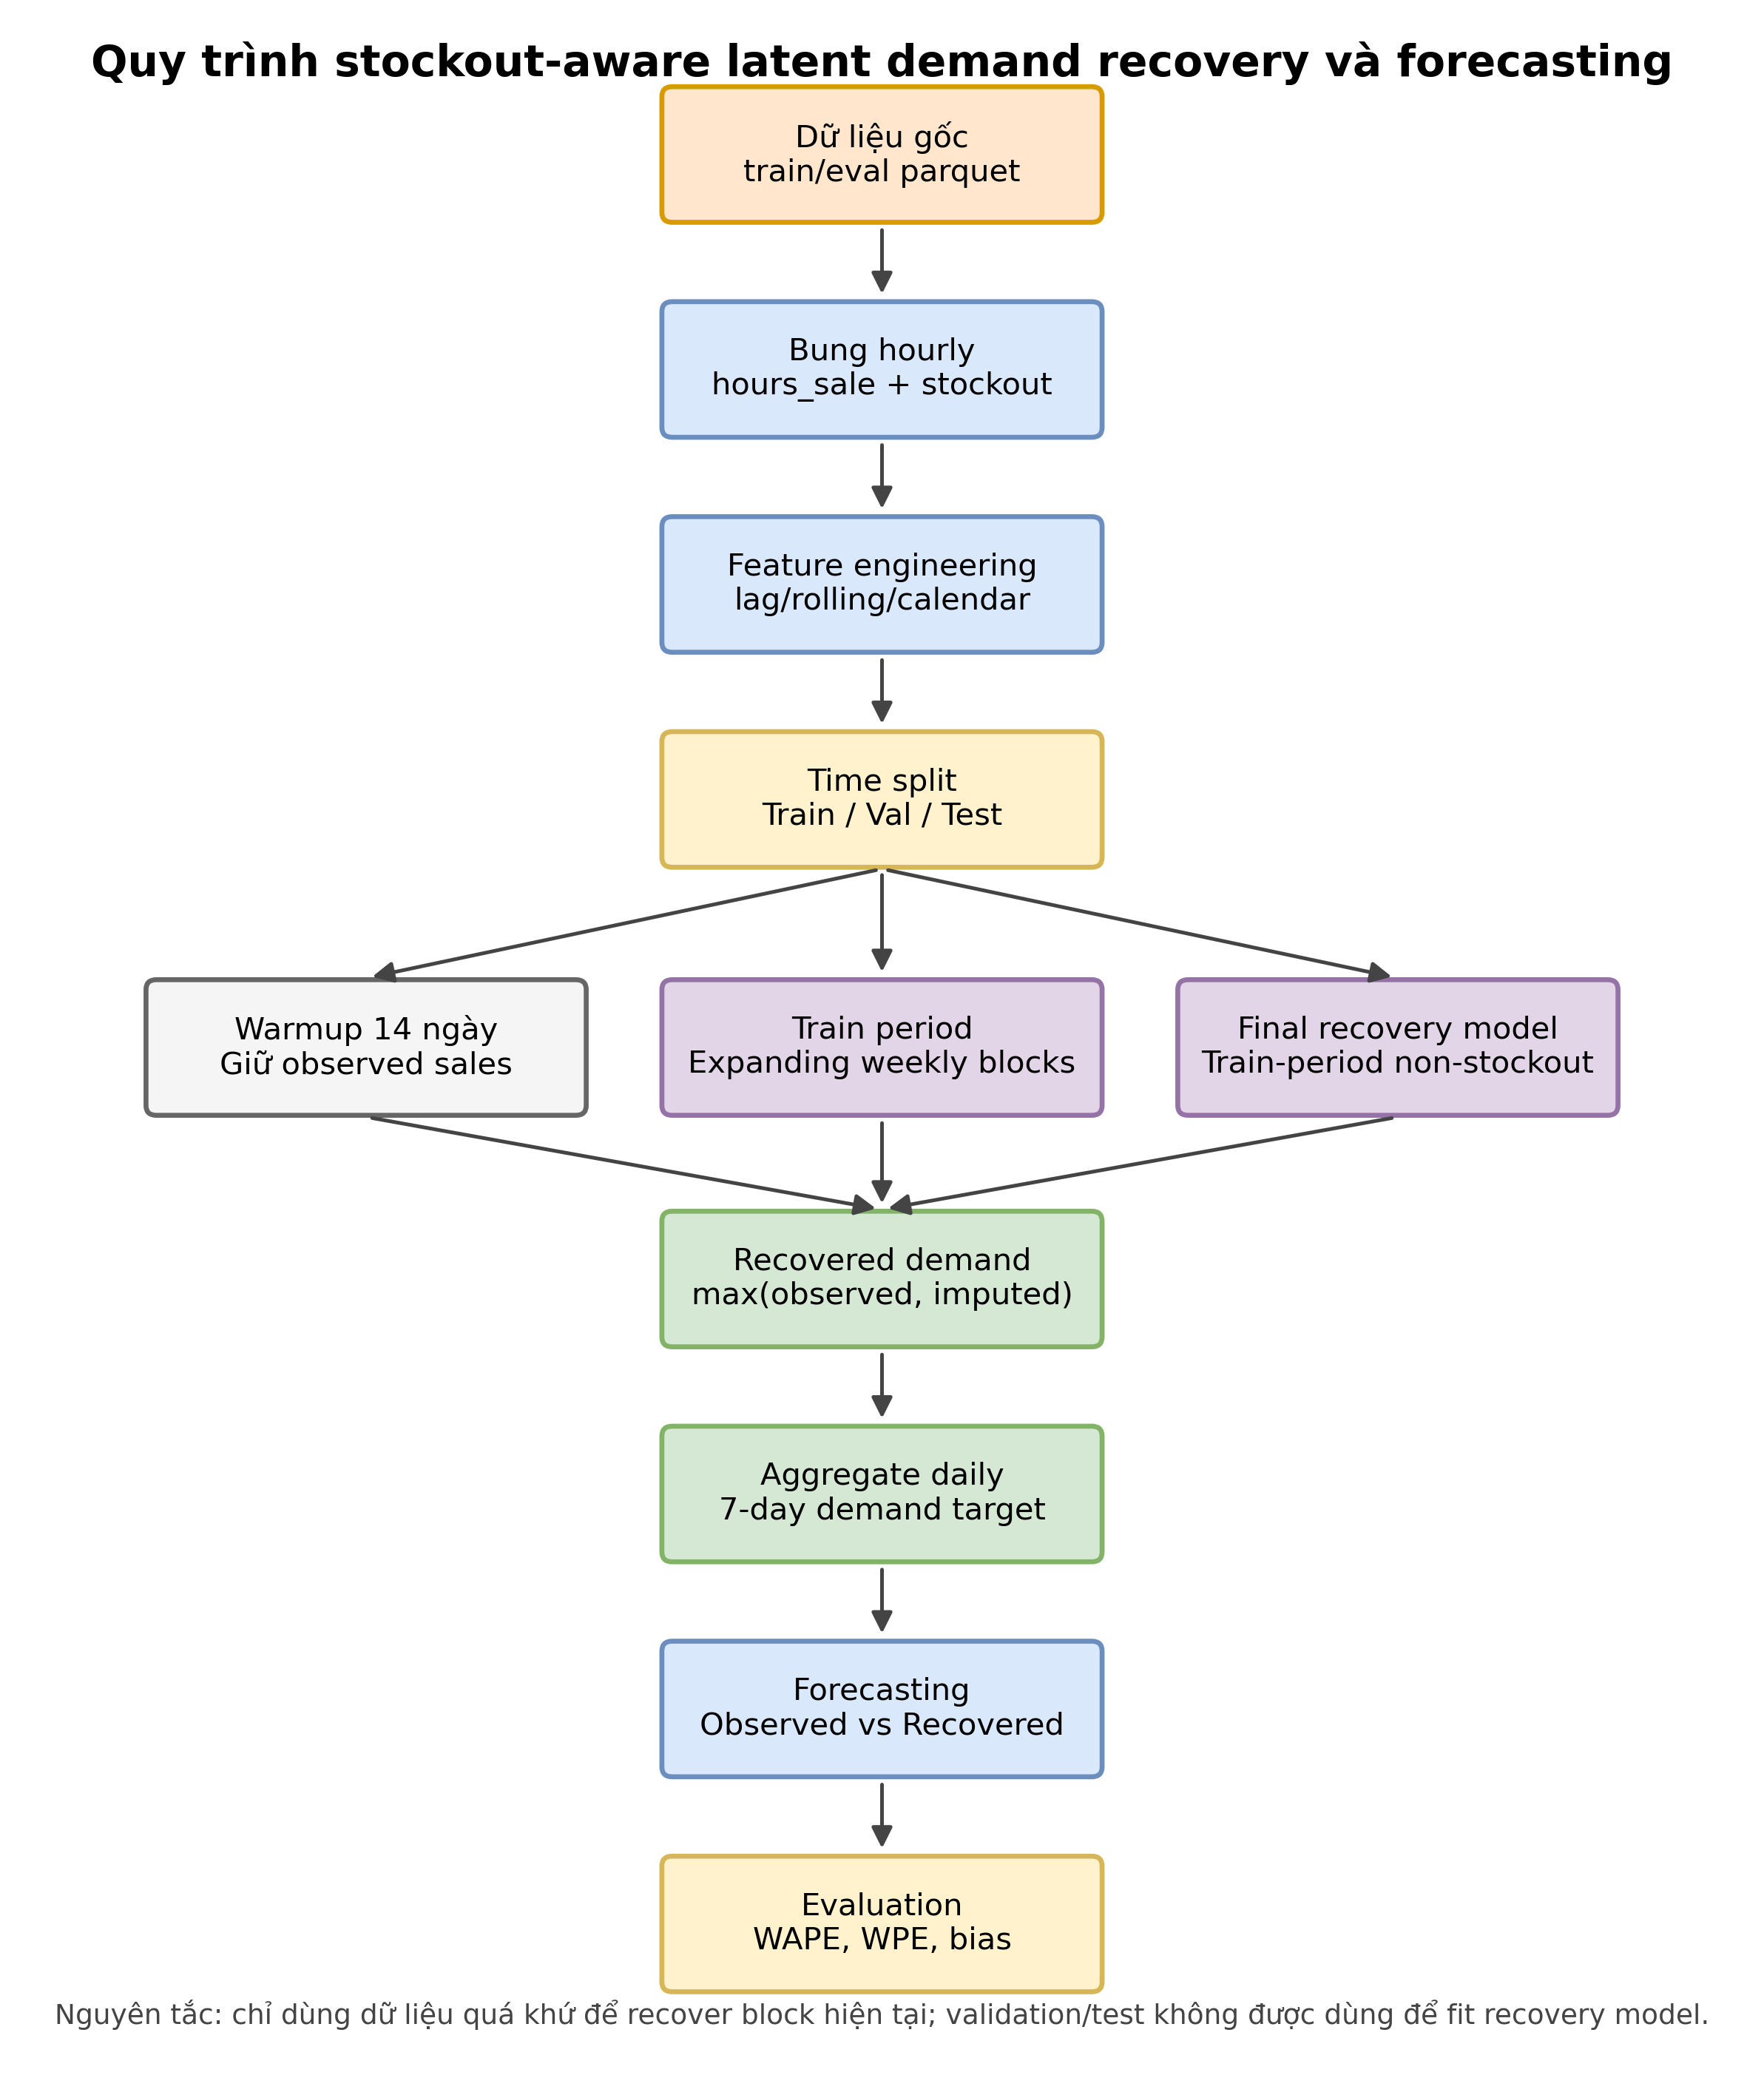
\includegraphics[width=0.92\linewidth,height=0.78\textheight,keepaspectratio]{owner_expanding_window_process.png}
\end{frame}

\begin{frame}{Expanding-window recovery chống leakage}
    \begin{columns}[T]
        \begin{column}{0.52\linewidth}
            \begin{itemize}
                \item Warm-up 14 ngày để có đủ hai chu kỳ tuần.
                \item Mỗi block 7 ngày chỉ học từ non-stockout rows trong quá khứ.
                \item Validation/test recovery chỉ dùng model fit từ train-period.
                \item Calibration cũng lấy từ train-period out-of-fold rows.
            \end{itemize}
            \begin{block}{Nguyên tắc}
            Không dùng ngày tương lai để recover nhu cầu của ngày quá khứ.
            \end{block}
        \end{column}
        \begin{column}{0.46\linewidth}
            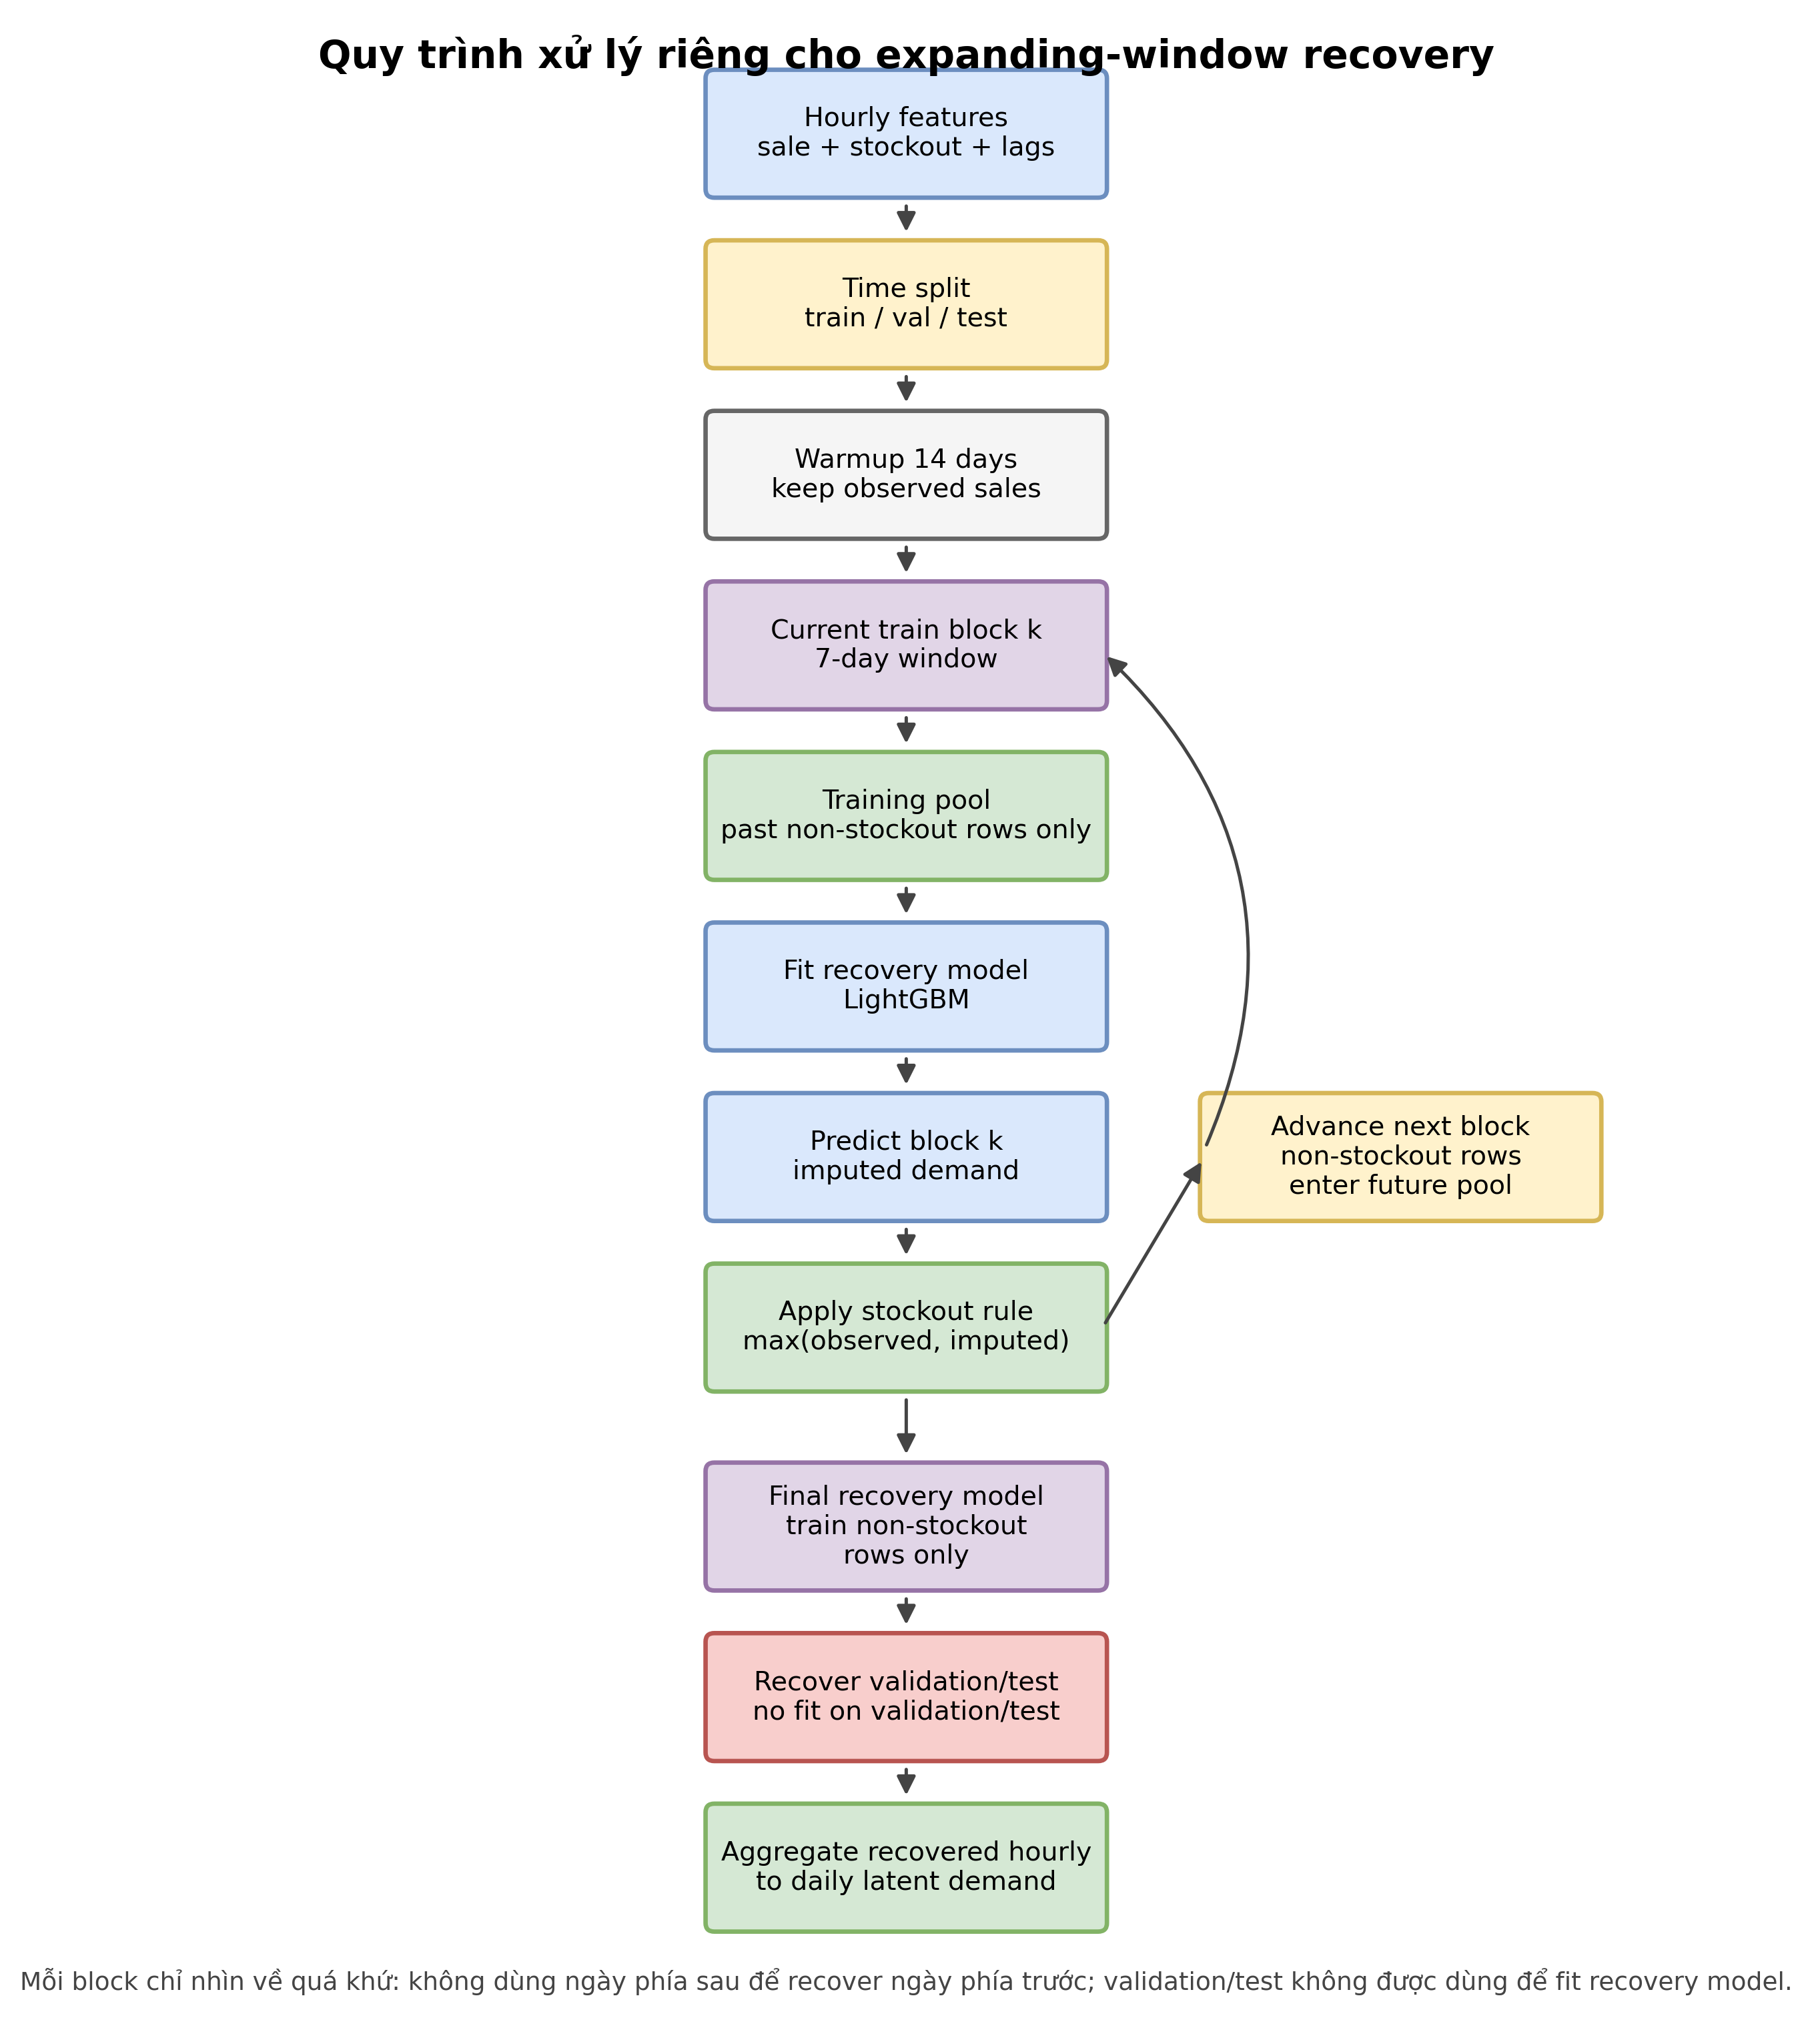
\includegraphics[width=\linewidth,height=0.66\textheight,keepaspectratio]{owner_expanding_window_recovery_detail.png}
        \end{column}
    \end{columns}
\end{frame}

\begin{frame}{Feature engineering: không chỉ lag của chính series}
    \small
    \begin{columns}[T]
        \begin{column}{0.49\linewidth}
            \textbf{Nhóm feature chính}
            \begin{itemize}
                \item Calendar: hour, day-of-week, month.
                \item Lag/rolling: 1, 7, 14, 28 ngày; 24/168 giờ.
                \item Stockout: flag, rate, rolling stockout.
                \item Promotion/weather/category/store/product.
            \end{itemize}
        \end{column}
        \begin{column}{0.49\linewidth}
            \textbf{Hai điểm mù được bổ sung}
            \begin{itemize}
                \item Velocity/momentum: bán nhanh trước stockout.
                \item Peer/substitution: sản phẩm cùng store/category.
                \item Mục tiêu: cho recovery nhìn thêm bối cảnh xung quanh stockout.
            \end{itemize}
        \end{column}
    \end{columns}
    \vspace{0.05cm}
    \centering
    \includegraphics[width=0.62\linewidth,height=0.28\textheight,keepaspectratio]{stockout_substitution_velocity_diagnostics.png}
\end{frame}

\begin{frame}{Imputation control: không để recovery phóng đại demand}
    \begin{columns}[T]
        \begin{column}{0.47\linewidth}
            \begin{tabular}{lr}
                \toprule
                Observed sales & 482,697.09 \\
                Recovered demand & 539,898.12 \\
                Recovered lost demand & 57,201.70 \\
                Lift & 11.85\% \\
                Calibration factor & 1.0110 \\
                Cap q90 & 0.0729 \\
                \bottomrule
            \end{tabular}
        \end{column}
        \begin{column}{0.50\linewidth}
            \begin{block}{Công thức}
            Raw impute $\rightarrow$ calibration $\rightarrow$ positive lost demand $\rightarrow$ cap q90 $\rightarrow$ recovered demand.
            \end{block}
            \begin{itemize}
                \item q90 giữ khoảng 78.88\% raw lost demand.
                \item q100 lift lên 15.02\% nhưng rủi ro over-imputation.
            \end{itemize}
        \end{column}
    \end{columns}
\end{frame}

\begin{frame}{Pseudo-stockout validation và sensitivity}
    \begin{columns}[T]
        \begin{column}{0.48\linewidth}
            \textbf{Pseudo-stockout validation}
            \begin{itemize}
                \item Dùng non-stockout rows trong validation làm ``đáp án giả''.
                \item Daily aggregate WAPE: 16.56\%.
                \item Prediction/actual ratio: 1.1152.
                \item Recovery còn hơi over-predict, nên cần cap.
            \end{itemize}
        \end{column}
        \begin{column}{0.50\linewidth}
            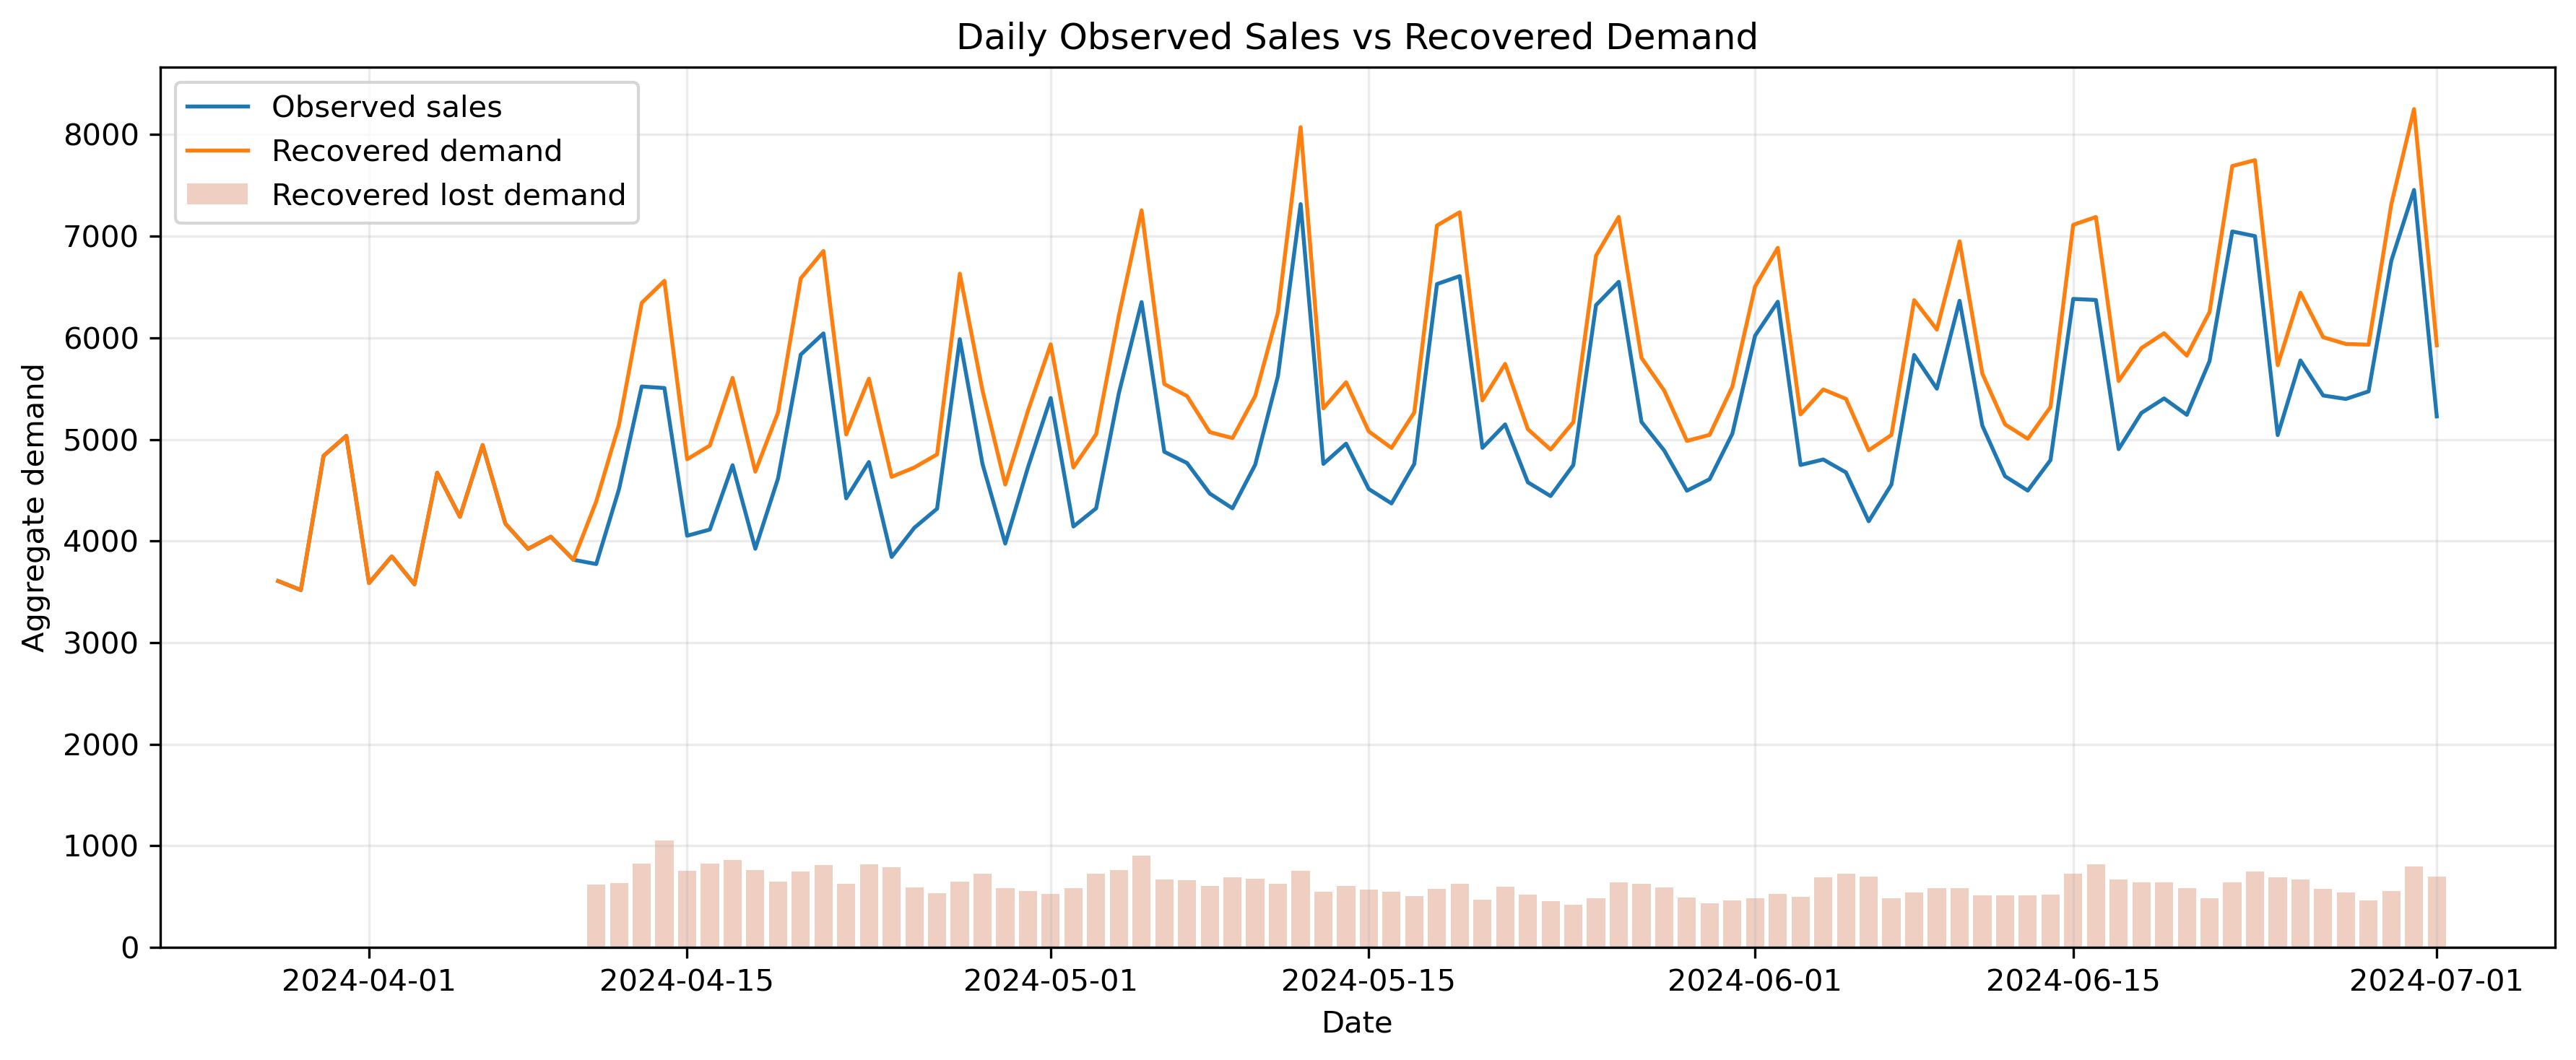
\includegraphics[width=\linewidth]{imputation_daily_uplift.png}
        \end{column}
    \end{columns}
\end{frame}

\section{Forecasting Results}
\begin{frame}{4. Forecasting setup}
    \begin{columns}[T]
        \begin{column}{0.50\linewidth}
            \textbf{Target}
            \begin{itemize}
                \item Hourly recovered demand $\rightarrow$ daily demand.
                \item Forecast origin ngày $t$.
                \item Target: tổng demand từ $t+1$ đến $t+7$.
            \end{itemize}
        \end{column}
        \begin{column}{0.48\linewidth}
            \textbf{Models}
            \begin{itemize}
                \item Naive x7.
                \item Seasonal naive 7-day.
                \item Observed-sales LightGBM.
                \item Recovered-demand LightGBM.
                \item Hybrid seasonal-ML.
            \end{itemize}
        \end{column}
    \end{columns}
    \vspace{0.2cm}
    \begin{block}{Evaluation}
    So sánh trên recovered latent demand proxy để trả lời đúng câu hỏi: forecast demand đã giảm bias do stockout.
    \end{block}
\end{frame}

\begin{frame}{Forecasting results: hybrid tốt nhất nhưng seasonal naive rất mạnh}
    \begin{columns}[T]
        \begin{column}{0.47\linewidth}
            \begin{tabular}{lrr}
                \toprule
                Model & WAPE & WPE \\
                \midrule
                Naive x7 & 31.46\% & -2.00\% \\
                Seasonal naive & 19.85\% & -6.12\% \\
                Observed LGBM & 24.92\% & -18.74\% \\
                Recovered LGBM & 20.19\% & -7.84\% \\
                Hybrid & 19.62\% & -7.15\% \\
                \bottomrule
            \end{tabular}
            \vspace{0.15cm}
            \begin{itemize}
                \item Hybrid giảm WAPE 21.27\% so với observed-sales LGBM.
            \end{itemize}
        \end{column}
        \begin{column}{0.51\linewidth}
            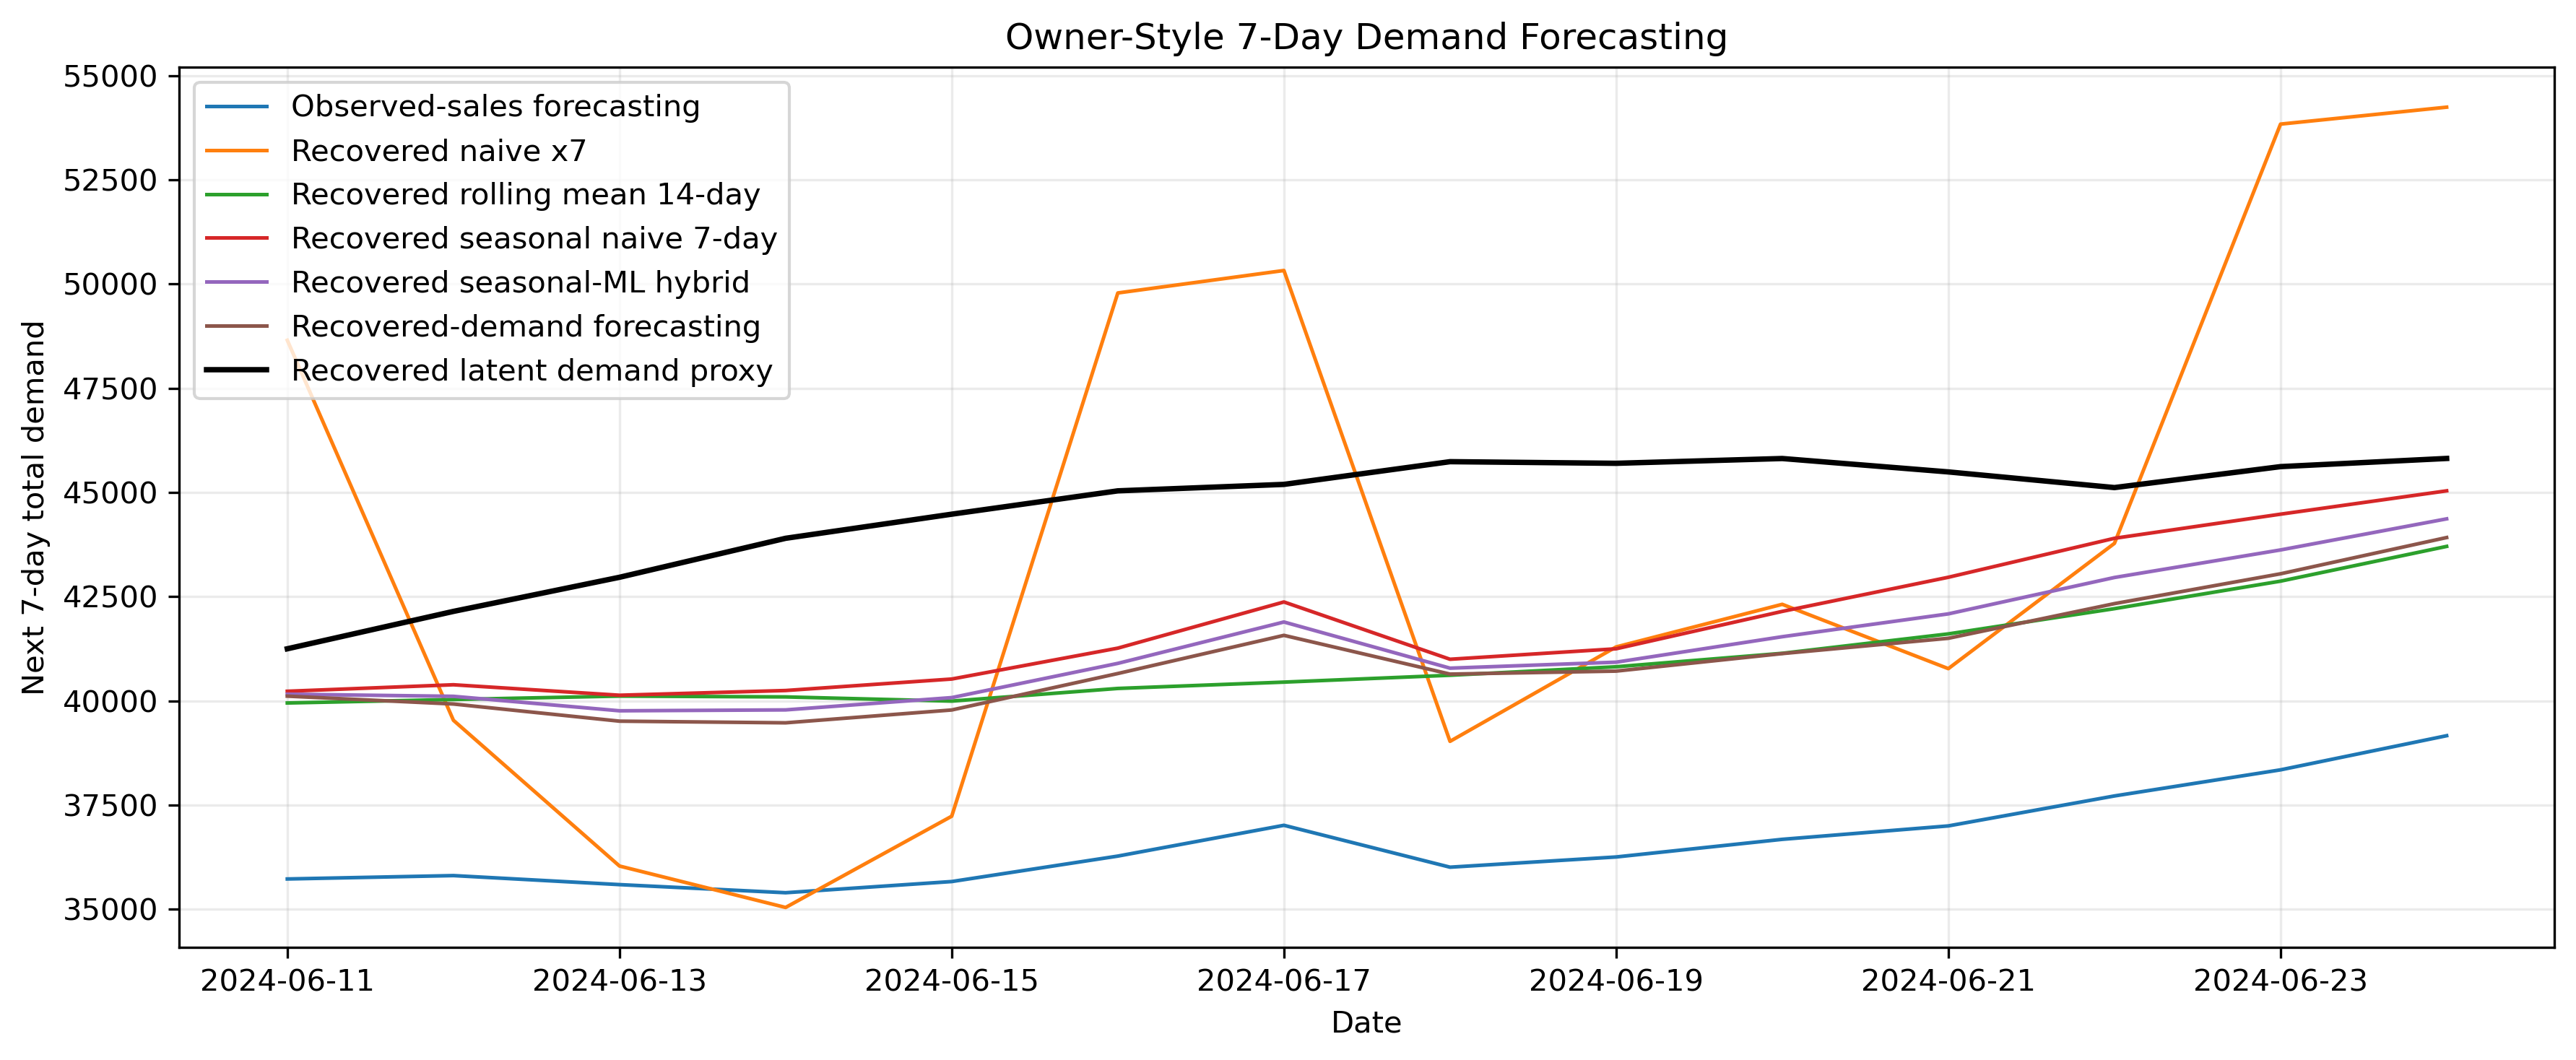
\includegraphics[width=\linewidth]{owner_two_stage_forecast_comparison.png}
        \end{column}
    \end{columns}
\end{frame}

\begin{frame}{Hybrid seasonal-ML là gì?}
    \begin{block}{Công thức kết hợp}
    $\hat{y}_{hybrid} = \alpha \hat{y}_{LightGBM} + (1-\alpha)\hat{y}_{SeasonalNaive}$
    \end{block}
    \begin{columns}[T]
        \begin{column}{0.49\linewidth}
            \textbf{Trọng số chọn bằng validation}
            \begin{itemize}
                \item LightGBM weight: 60\%.
                \item Seasonal naive weight: 40\%.
                \item Không chọn bằng test set.
            \end{itemize}
        \end{column}
        \begin{column}{0.49\linewidth}
            \textbf{Tại sao hợp lý?}
            \begin{itemize}
                \item Seasonal naive giữ pattern tuần.
                \item LightGBM hiệu chỉnh theo stockout, lag, product/store.
                \item Giảm rủi ro ML học quá phức tạp nhưng thua baseline.
            \end{itemize}
        \end{column}
    \end{columns}
\end{frame}

\begin{frame}{Feature importance: mô hình học gì?}
    \begin{columns}[T]
        \begin{column}{0.47\linewidth}
            \begin{itemize}
                \item \texttt{stockout\_rate} là feature quan trọng nhất.
                \item Lag 7/14/28 ngày xác nhận weekly pattern.
                \item Rolling mean/sum giúp ổn định chuỗi thưa.
            \end{itemize}
            \begin{block}{Diễn giải}
            Model không chỉ dựa vào trend gần nhất; nó kết hợp stockout, seasonality và lịch sử demand đã recover.
            \end{block}
        \end{column}
        \begin{column}{0.51\linewidth}
            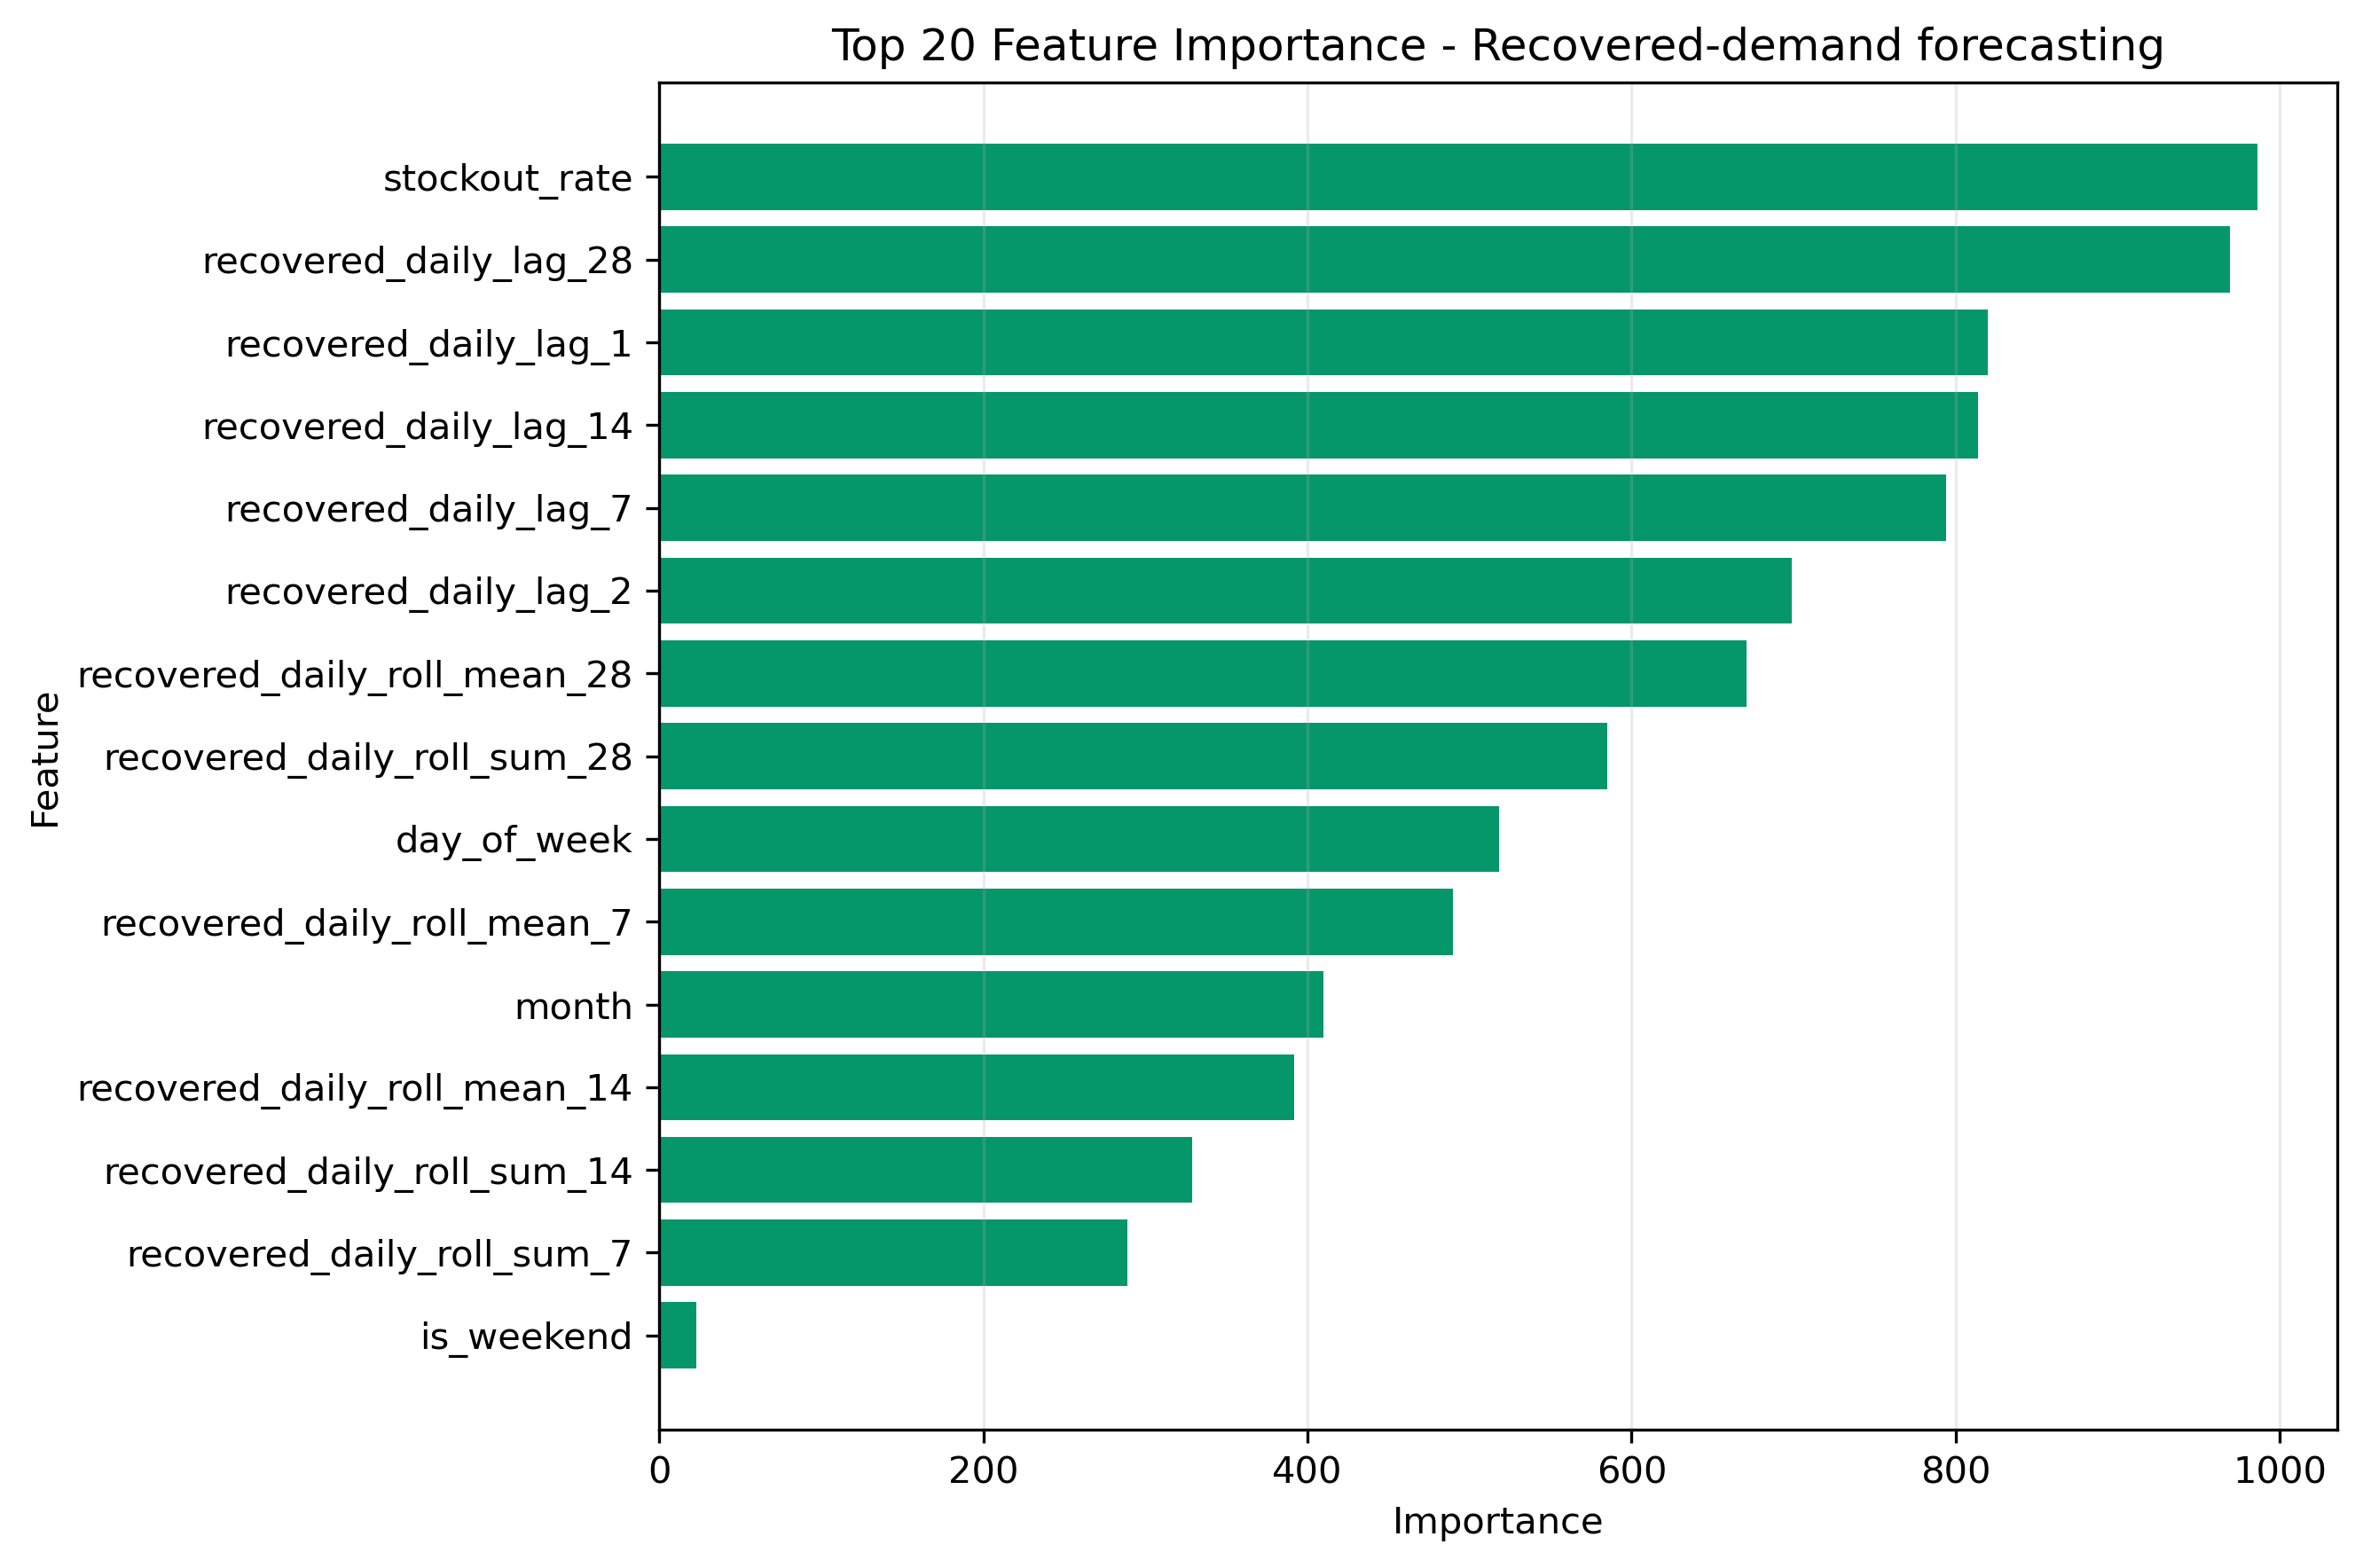
\includegraphics[width=\linewidth]{owner_recovereddemand_forecasting_feature_importance_top20.png}
        \end{column}
    \end{columns}
\end{frame}

\section{Model Evaluation}
\begin{frame}{5. Model evaluation: residual diagnostics}
    \begin{columns}[T]
        \begin{column}{0.49\linewidth}
            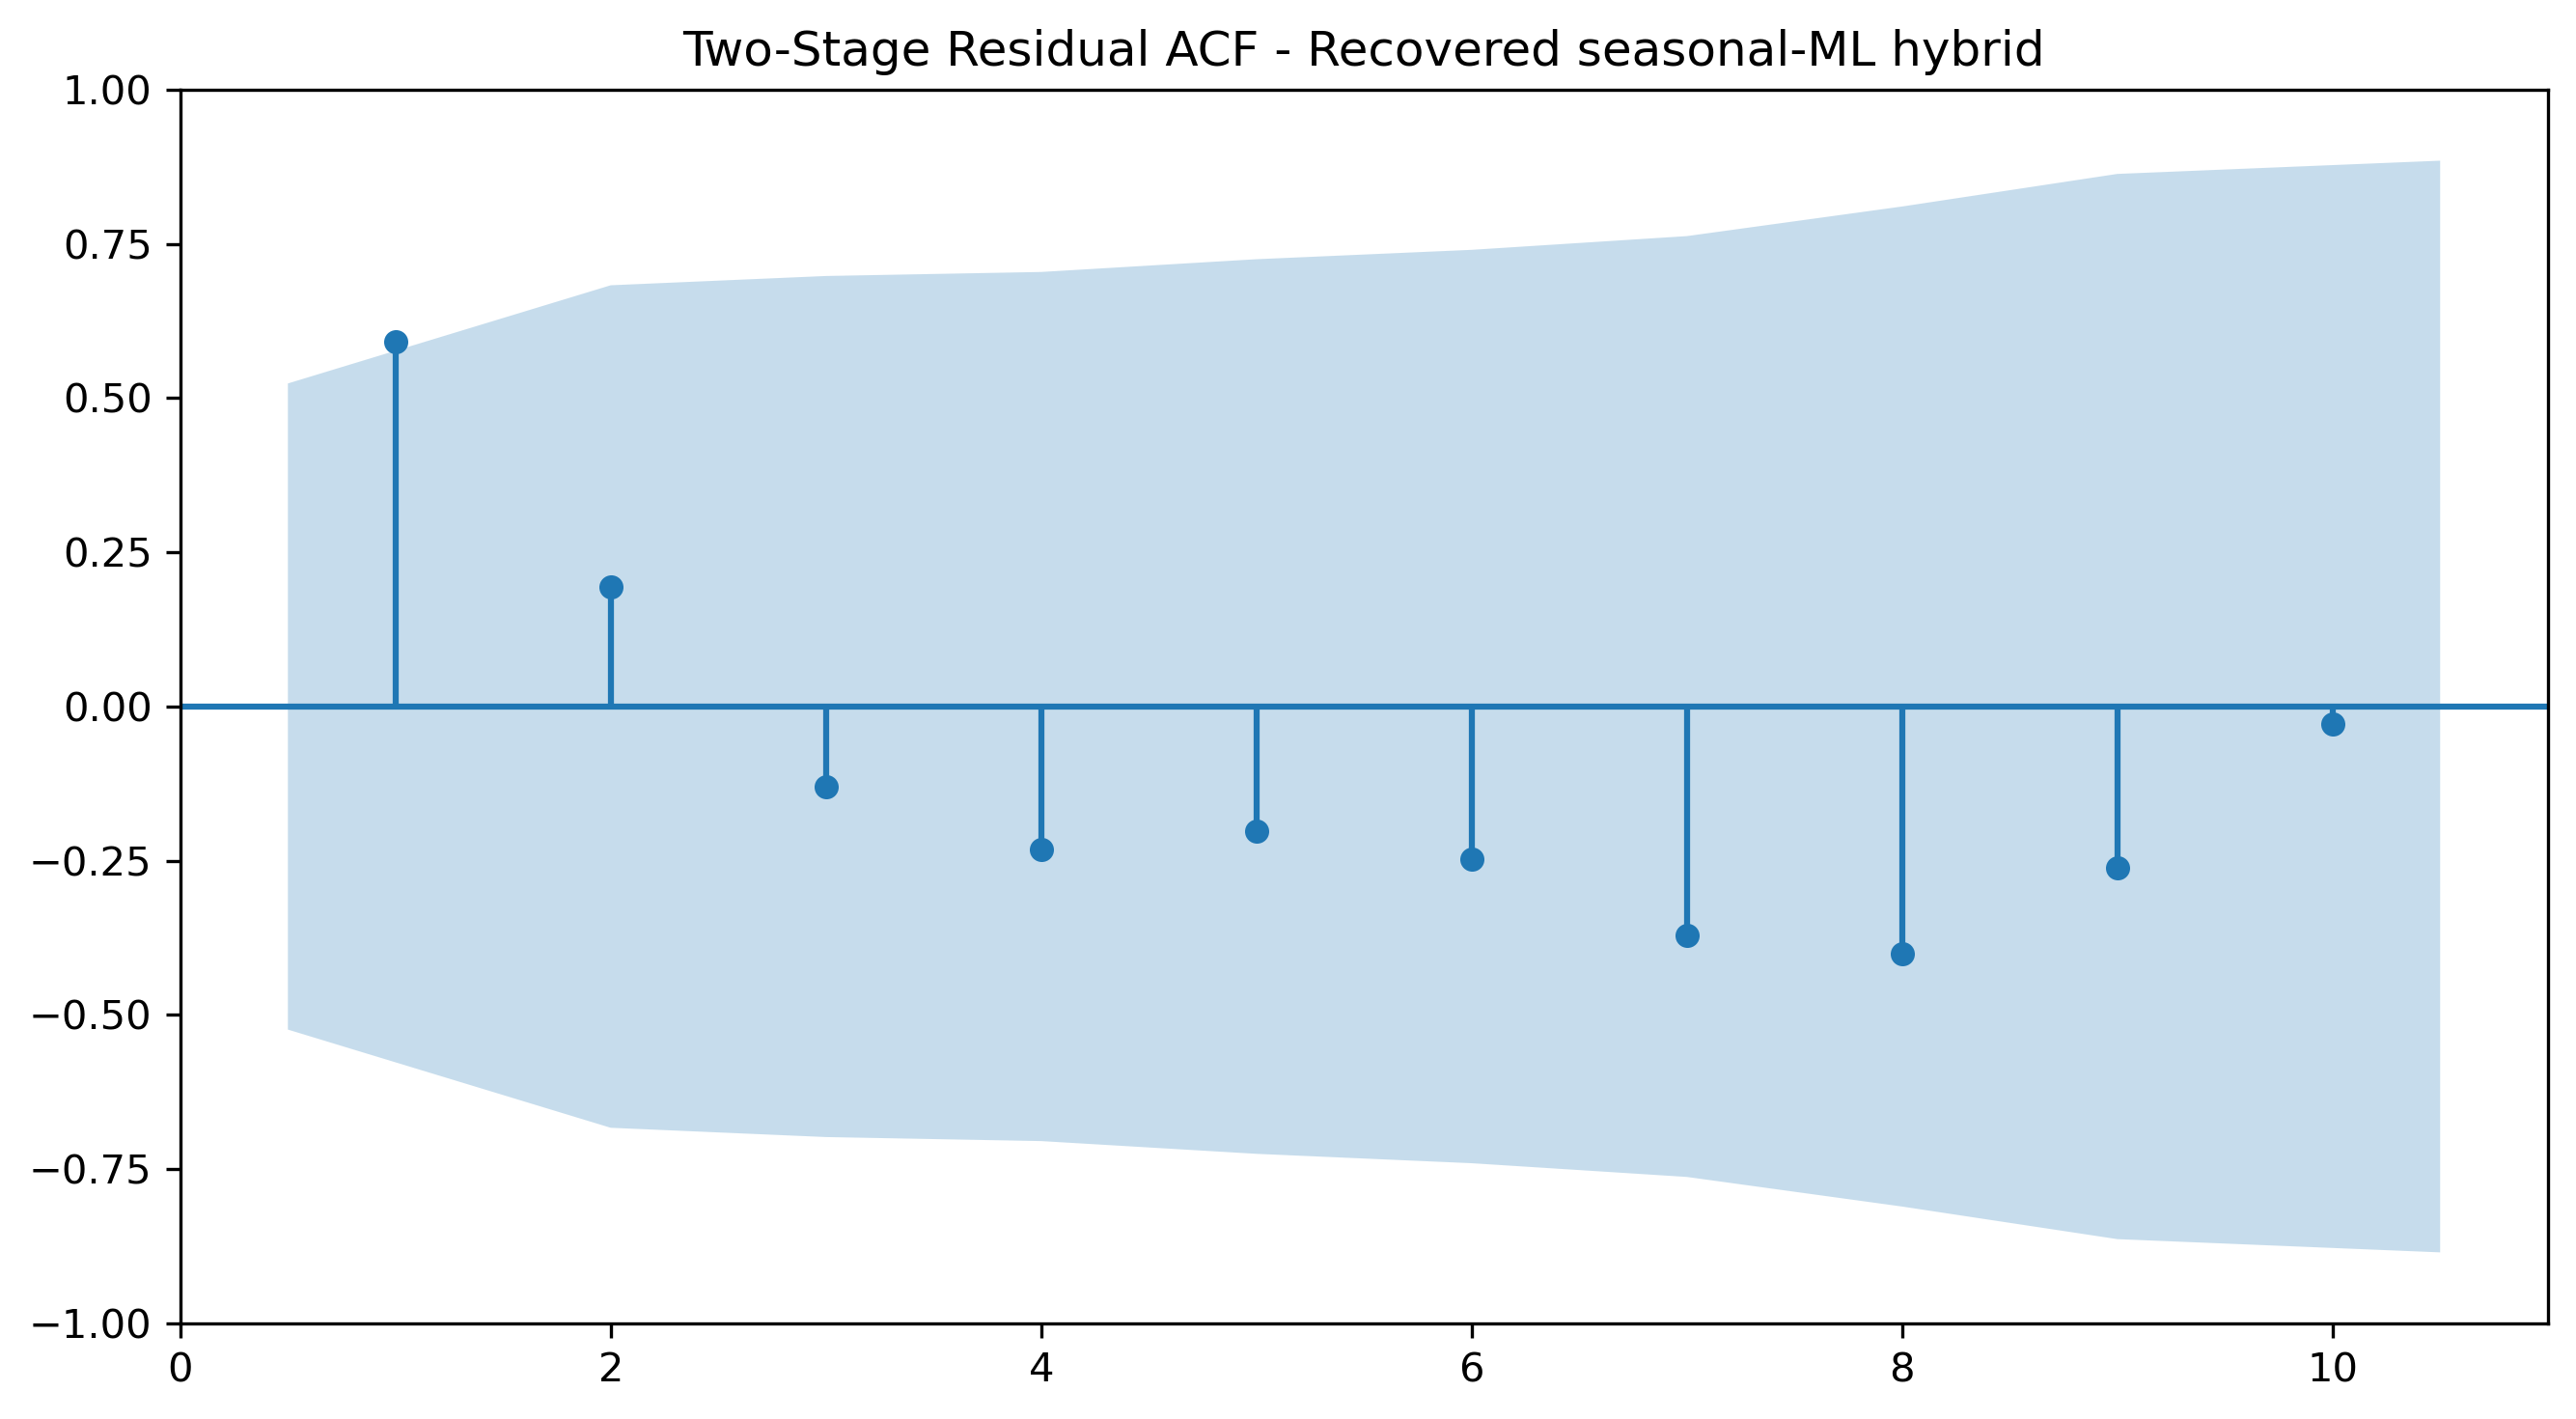
\includegraphics[width=\linewidth]{owner_two_stage_residual_acf.png}
        \end{column}
        \begin{column}{0.49\linewidth}
            \begin{itemize}
                \item Hybrid Ljung--Box p-value: 0.0288.
                \item Residual chưa hoàn toàn white noise.
                \item Một phần do target next-7-day bị overlap.
                \item Kết luận trung thực: model cải thiện forecast nhưng chưa học hết pattern.
            \end{itemize}
        \end{column}
    \end{columns}
\end{frame}

\begin{frame}{Prediction intervals: forecast không phải một con số chắc chắn}
    \begin{columns}[T]
        \begin{column}{0.48\linewidth}
            
\includegraphics[width=\linewidth]{owner_two_stage_forecast_interval.png}
        \end{column}
        \begin{column}{0.49\linewidth}
            \begin{tabular}{lr}
                \toprule
                Hybrid 80\% coverage & 76.77\% \\
                Hybrid 95\% coverage & 93.89\% \\
                Mean 80\% width & 4.43 \\
                Mean 95\% width & 9.78 \\
                \bottomrule
            \end{tabular}
            \vspace{0.2cm}
            \begin{itemize}
                \item 80\% interval hơi hẹp.
                \item 95\% interval phù hợp hơn nhưng rộng hơn.
                \item Dùng để chọn safety stock theo rủi ro.
            \end{itemize}
        \end{column}
    \end{columns}
\end{frame}

\section{Business Insights}
\begin{frame}{6. Business insights: lost sales và ưu tiên vận hành}
    \begin{columns}[T]
        \begin{column}{0.49\linewidth}
            
\includegraphics[width=\linewidth]{imputation_top_series_lift.png}
        \end{column}
        \begin{column}{0.49\linewidth}
            \textbf{Insight}
            \begin{itemize}
                \item Recovered lost demand: 57,201.70.
                \item Lift over observed: 11.85\%.
                \item Không phải mọi stockout quan trọng như nhau.
                \item Ưu tiên series có uplift/lost demand cao.
            \end{itemize}
            \begin{block}{Hành động}
            Kiểm tra safety stock, lead time, tần suất bổ sung và chất lượng ghi nhận stock status ở nhóm uplift cao.
            \end{block}
        \end{column}
    \end{columns}
\end{frame}

\begin{frame}{Ứng dụng vào replenishment}
    \begin{center}
    \begin{tabular}{p{0.23\linewidth}p{0.30\linewidth}p{0.34\linewidth}}
        \toprule
        Bước & Đầu vào & Đầu ra vận hành \\
        \midrule
        Recovery & Hourly sales + stockout & Recovered demand proxy \\
        Forecast & Daily recovered demand & Next-7-day demand \\
        Quy đổi nhập hàng & Forecast + tồn kho + lead time & Đề xuất lượng nhập \\
        Theo dõi & Actual + stockout + error & Cảnh báo bias/drift \\
        \bottomrule
    \end{tabular}
    \end{center}
    \vspace{0.15cm}
    \begin{columns}[T]
        \begin{column}{0.49\linewidth}
            \textbf{Nếu chi phí stockout cao}
            \begin{itemize}
                \item Dùng forecast gần upper interval.
                \item Tăng safety stock cho nhóm uplift cao.
            \end{itemize}
        \end{column}
        \begin{column}{0.49\linewidth}
            \textbf{Nếu hàng dễ hư hỏng}
            \begin{itemize}
                \item Dùng point forecast hoặc interval thấp hơn.
                \item Tăng tần suất cập nhật forecast.
            \end{itemize}
        \end{column}
    \end{columns}
\end{frame}

\section{Conclusion}
\begin{frame}{7. Conclusion}
    \begin{enumerate}
        \item Stockout làm observed sales đánh giá thấp demand, nên cần recovery trước forecast.
        \item Expanding-window recovery giúp tránh leakage theo thời gian.
        \item Recovered demand lift khoảng 11.85\% so với observed sales.
        \item Forecast trên recovered demand tốt hơn forecast trực tiếp observed sales.
        \item Hybrid seasonal-ML đạt WAPE 19.62\% và giữ được weekly pattern mạnh.
    \end{enumerate}
    \vspace{0.2cm}
    \begin{block}{Câu chốt}
    Điểm mạnh của đồ án là pipeline có kiểm soát: đúng framing, có benchmark mạnh, có diagnostics, có uncertainty và có business interpretation.
    \end{block}
\end{frame}

\begin{frame}{Limitations: nói rõ để bảo vệ tốt hơn}
    \begin{itemize}
        \item Recovered demand là proxy, không phải ground truth tuyệt đối.
        \item Pseudo-stockout validation còn over-predict nhẹ.
        \item Residual chưa white noise hoàn toàn.
        \item Peer/substitution mới ở mức feature đơn giản.
        \item Sample 10\% có thể chưa phản ánh đầy đủ toàn bộ network sản phẩm.
        \item Chưa triển khai deep imputation do phạm vi và tài nguyên đồ án.
    \end{itemize}
    \vspace{0.2cm}
    \begin{block}{Tinh thần trình bày}
    Không giấu vấn đề; dùng diagnostics để biết mô hình còn sai ở đâu và vì sao.
    \end{block}
\end{frame}

\section{Future Work}
\begin{frame}{8. Future work}
    \begin{columns}[T]
        \begin{column}{0.50\linewidth}
            \textbf{Kỹ thuật}
            \begin{itemize}
                \item Deep imputation: SAITS, CSDI, TimesNet, ImputeFormer.
                \item Product substitution graph.
                \item Quantile/conformal forecasting.
                \item Rolling retraining và drift monitoring.
            \end{itemize}
        \end{column}
        \begin{column}{0.48\linewidth}
            \textbf{Business evaluation}
            \begin{itemize}
                \item Giảm stockout rate.
                \item Giảm lost sales proxy.
                \item Kiểm soát hàng hủy/tồn kho dư.
                \item A/B test theo store/category.
            \end{itemize}
        \end{column}
    \end{columns}
    \vspace{0.2cm}
    \begin{block}{Nguyên tắc mở rộng}
    Model phức tạp hơn chỉ đáng dùng nếu vượt seasonal baseline và giữ được validation chống leakage.
    \end{block}
\end{frame}

\begin{frame}{Cảm ơn}
    \centering
    \vspace{1cm}
    {\Large Cảm ơn thầy và các bạn đã lắng nghe!}\\[0.5cm]
    {\large Q\&A}\\[0.8cm]
    \begin{block}{Một câu nhớ nhất}
    Forecast tốt trong bài này không bắt đầu từ model phức tạp, mà bắt đầu từ việc hiểu đúng observed sales bị stockout censor.
    \end{block}
\end{frame}

\end{document}
